%
\begin{figure*}
  \centering
  %!TEX root = ../../14-icra-RealTimeNMPC.tex

\tikzstyle{block} = [draw, fill=blue!20, rectangle,
    minimum height=2em, minimum width=5em, align=center]
\tikzstyle{sum} = [draw, fill=blue!20, circle, node distance=1cm]
\tikzstyle{input} = [coordinate]
\tikzstyle{output} = [coordinate]
\tikzstyle{pinstyle} = [pin edge={to-,thin,black}]

% The block diagram code is probably more verbose than necessary
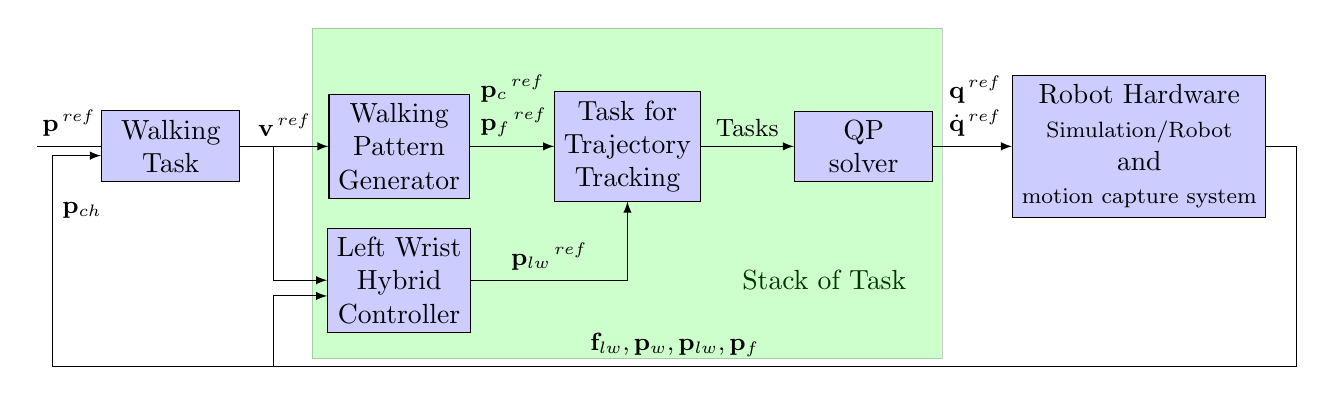
\begin{tikzpicture}[auto, node distance=2cm,>=latex]

    % We start by placing the blocks
    \node [input]  at (0.0, 0.0) (input)  {};
    \node [input]  at (3, 0.0) (velocity) {};
    \node [input]  at (0.2, -2.8) (feedback)  {};
    \node [input]  at (16, -2.8) (feedback2)  {};
    \node []    at ( 0.0, 0.0) (sumin)  {};
    %\node [output]    at ( 15, 0.0) (sumout) {};
    \draw [fill=green,opacity=.2,text opacity=1] (3.5,1.5) rectangle (11.5,-2.7);
    \node at(10,-1.7) {\textcolor{green!20!black!100}{Stack of Task}};

    \node [block] at (4.6,-1.7) (lwc) {
        Left Wrist\\
        Hybrid\\
        Controller        
    };

    \node [block] at (1.7,0.0) (walking) {
        Walking \\
        Task    
    };

    \node [block] at (4.6,0) (wpg) {
        Walking\\
        Pattern\\
        Generator
    };
%    \node [block] at (4.2,0) (dyn) {
%        Dynamic\\
%        Filter
%    };
    \node [block] at (7.5,0) (ttt) {
        Task for\\
        Trajectory\\
        Tracking
    };
    
    \node [block] at (10.5,0) (qp) {
        QP\\
        solver
    };

    \node [block] at (14.0, 0) (system) {
    		Robot Hardware\\
    		{\footnotesize Simulation/Robot}\\
    		and\\
    		{\footnotesize motion capture system}
    	};

    % PATHS
    	% Forward chaine
    \draw [draw,-] (input) -- node {\small ${\mathbf{p}}^{\,{\text {ref}}}$} (walking);
    
    \draw [draw,->] (walking) -- node {\small ${\mathbf v}^{\,{\text{ref}}}$} (wpg);
%    \draw [draw,- ] (walking) -- node {} (velocity);
    \draw [draw,->] (velocity) |- node {} (lwc);
%    \draw [->] (wpg) -- node {\small $c^{ref},f^{ref}$} (dyn);
%    \draw [->] (dyn) -- node {\small $\tilde{c}^{\,ref},f^{ref}$} (sot);
    \draw [->] (wpg) -- node [text width=0.8cm]{\small ${\mathbf{p}_c}^{\,{\text {ref}}}$ ${\mathbf{p}_f}^{\,{\text {ref}}}$} (ttt);
    \draw [->] (ttt) -- node [text width=0.8cm]{
    \small Tasks
    } (qp);
    \draw [->] (qp) -- node [text width=0.6cm]{\small ${\mathbf q}^{\,{\text{ref}}}$ $\dot{{\mathbf q}}^{\,{\text{ref}}}$} (system);
    
    \draw [->] (lwc) -| node [near start, above]{\small ${\mathbf{p}_{lw}}^{\,{\text {ref}}}$} (ttt);
    %\draw [->] (system) -- node {} (sumout);

    % Feedback chaine
%    \draw [- ] (dyn)      -| node {} (feedback);
%    \draw [->] (feedback) -| node {} (wpg);
    
    \draw [- ] (system.east)    -| node {} (feedback2);
    \draw [- ] (feedback2)  -- node [above]{\small $\mathbf{f}_{lw},\mathbf{p}_{w},\mathbf{p}_{lw},\mathbf{p}_{f}$} (feedback);
    \draw [->] (3.0,-2.8) |- node [near start, above]{} ([yshift=-0.2cm]lwc.west);
    \draw [->] (feedback) |- node [below=0.7cm, right]{\small $\mathbf{p}_{ch}$} ([yshift=-0.2cm]walking);

%    \draw [->] (dyn) -| node[above right] {\small $\hat{c}^{\,x,y,\theta}$, $\hat{f}^{\,\,x,y,\theta}$} (wpg);
\end{tikzpicture}
\caption[Control scheme for pulling a stiff hose]{This scheme describe the feedback loop used to control the humanoid robot HRP-$2$. With ${\mathbf{p}}^{\,{\text {ref}}}$ as the user defined pose, ${\mathbf{v}}^{\,{\text {ref}}}$ as the velocity computed from the walking task, ${\mathbf{p}_c}^{\,{\text {ref}}}$ as the center of mass reference trajectory, ${\mathbf{p}_f}^{\,{\text {ref}}}$ as the feet reference trajectories, ${\mathbf q}^{\,{\text{ref}}},\dot{{\mathbf q}}^{\,{\text{ref}}}$ being respectively the generalized position and velocity vector, ${\mathbf{p}_{lw}}^{\,{\text {ref}}}$ as the reference left wrist position, $\mathbf{f}_{lw},\mathbf{p}_{w},\mathbf{p}_{lw},\mathbf{p}_{f},\mathbf{p}_{ch}$ being respectively the measures of the left wrist force sensor, the waist position, the left wrist position, the feet position and the chest position.}

 \vspace{-3mm}
 \label{feed_back_graph}
\end{figure*}
%

%In this section the experimental results of the picking motion explained in section \ref{sec_pick} and the proposed strategy for pulling a fire hose with the HRP-$2$ humanoid robot are presented.


In Fig.~\ref{feed_back_graph}, the feedback control loop used in the experiments is shown.
%
The walking task uses the robot's chest position given by the motion capture system to compute the reference velocity $\mathbf{v}_{\text{ref}}$ for the walking pattern generator.
%
$\mathbf{v}_{\text{ref}}$ is also used by the impedance controller to compute the pulling force to be applied.
%
The reference positions for the feet and the center of mass are computed by the walking pattern generator, and the reference position of the left wrist is computed by the hybrid controller.
%
These reference positions are sent to a generalized inverse kinematics framework \cite{mansard:icar:09} that will compute the robot's joints angles reference trajectories to be executed by the robot.
%
The control framework uses the robot's forward kinematics to compute the current positions of the robot bodies, and the force sensors information to feedback the system.



The fire hose used in this work has a weight of $1.8$ kg/m, and a total length of $30$ meters.
%
There is no water inside.
%
It is empty and rolled up into a reel which is fixed to the floor, as shown in Fig.~\ref{rob_hose}(a).
%
For the picking experiment, the nozzle of the fire hose lays on the floor as shown in Fig.~\ref{exp_pick}(a) where the robot is at its half sitting configuration, i.e. its starting posture.
%
Fig.~\ref{exp_pick}(b) shows the robot posture at the picking time.
%
It can be seen that the robot successfully reaches the hose laid on the floor, without losing balance and without any self-collisions.



For the walking experiment the robot will pull the hose only in its forward walking direction, i.e. the diagonal elements of matrix $\mathbf{W}$ in equation (\ref{fpull}) are $w_{11} = \beta$, $w_{22} = 0.0$, and $w_{33}=0.0$, where $\beta$ is a constant.
%
%
\begin{figure}[t]
 \centering
 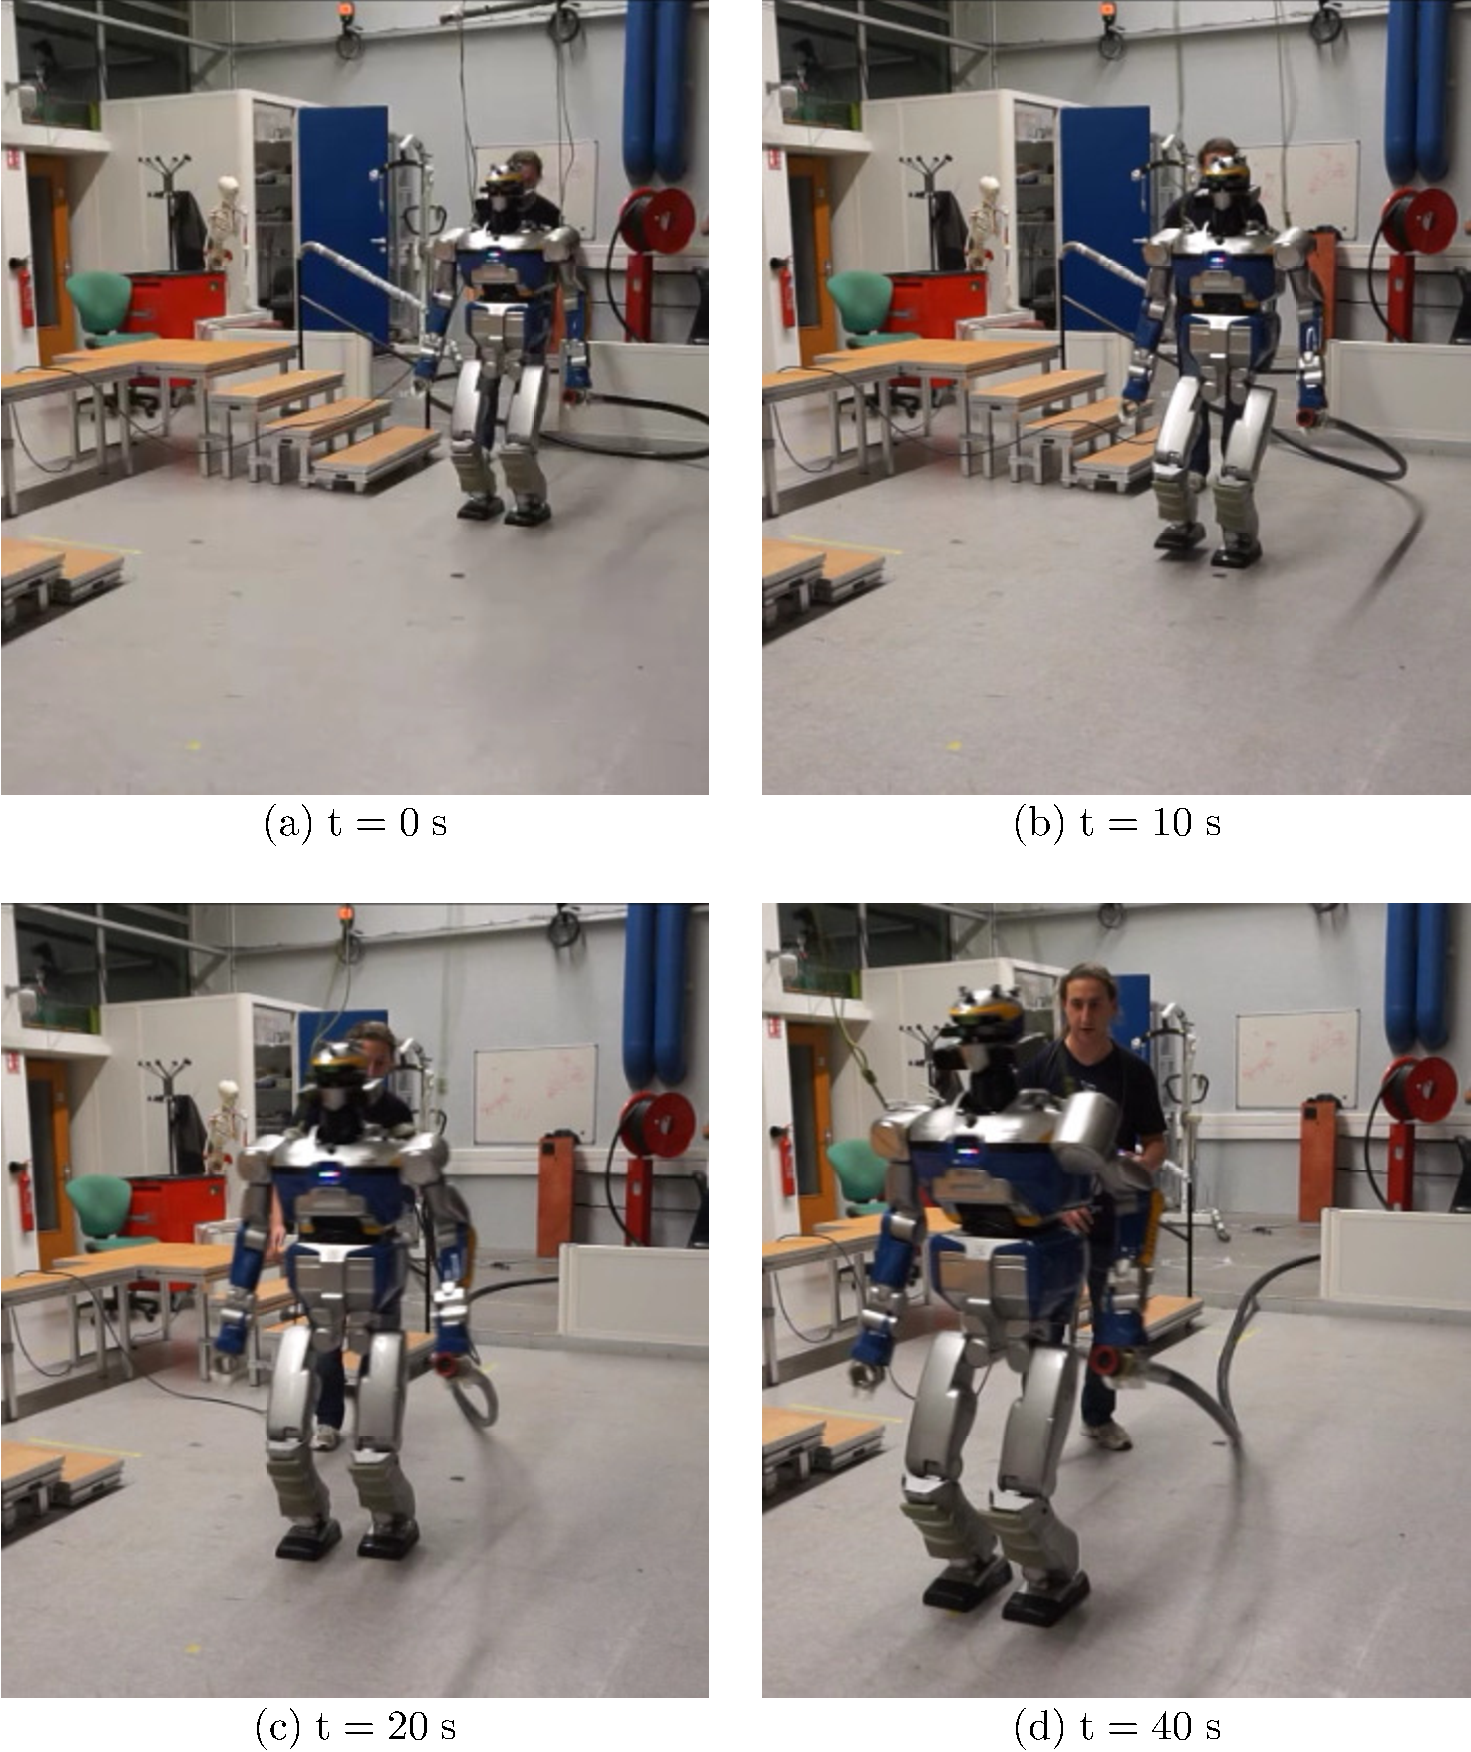
\includegraphics[height=0.40\textwidth]{./figures/exp_pics.pdf}
 \vspace{-3mm}
 \caption{Snapshots of the experiment on the HRP-$2$ robot pulling a fire hose.}
 \label{exp_pics}
% \vspace{-5mm}
\end{figure}
%
%
Using a motion capture system composed of $10$ infrared cameras (Motion Analysis Corp. \cite{mocap}), the position of the robot's chest is tracked on real time, with a sampling frequency of $200$ Hz.
%
The robot's starting position is $x_c = -1.1$ m, $y_c = 1.56$ m and the desired position given to the walking task is $\mathbf{x}_d = [1.0 \; 1.5 \; 0.0]^T$ with a tolerance of $5$ cm in $X$ and $Y$ direction and $5$ deg for the yaw angle.
%
This means that the robot will stop walking when all of the errors are within the tolerance value.
%
The walking task is set with a maximal velocity of $0.1$ and $0.15$ m/step for the $X$ and $Y$ directions, respectively, and $5$ deg/step.
The step duration is fixed and lasts $0.8$ s.
%
Fig.~\ref{exp_pics} shows snapshots of the experiment carried out on the HRP-$2$ humanoid robot, and Fig.~\ref{exp_graph} shows the corresponding robot's chest trajectory tracked by the motion capture system.\footnote{The video of the experiment can be found in the multimedia attachment.}
%
%
\begin{figure}[t]
 \centering
 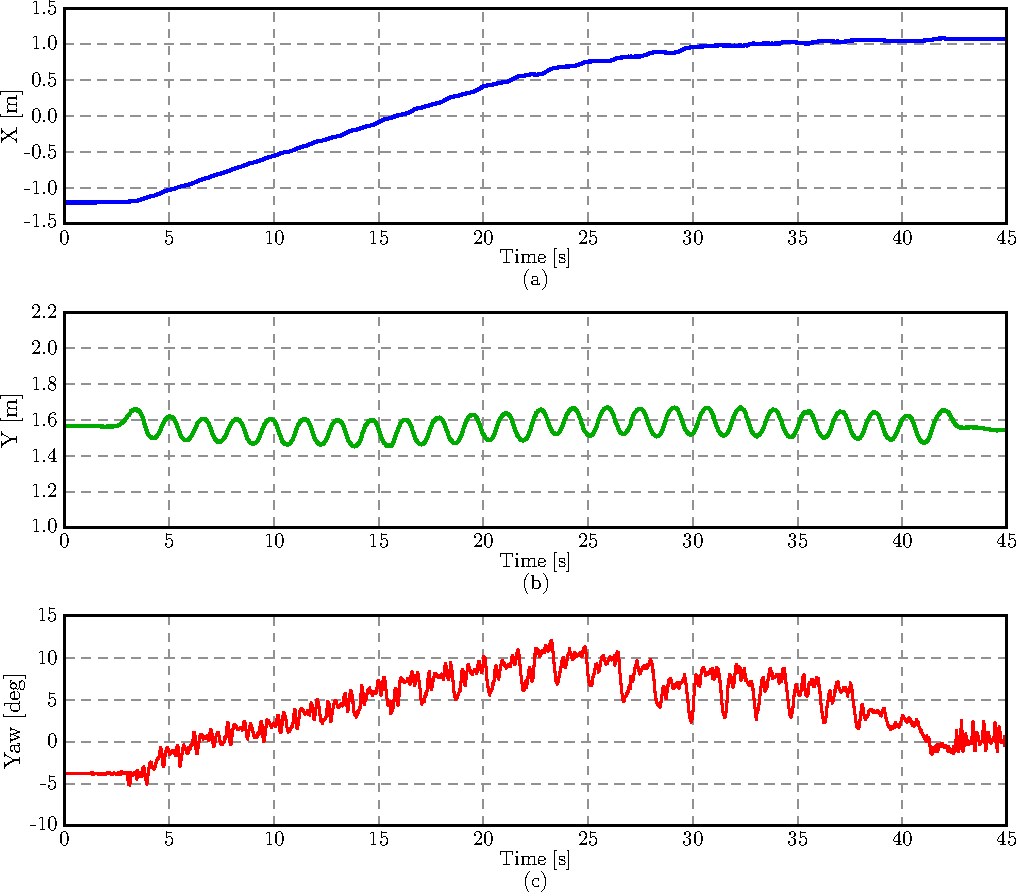
\includegraphics[height=0.40\textwidth]{./figures/exp_pos.pdf}
 \vspace{-3mm}
 \caption{Robot's chest trajectory in experiment. In (a) position in $X$ direction, in (b) position in $Y$ direction and in (c) yaw angle.}
 \label{exp_graph}
% \vspace{-5mm}
\end{figure}
%
%
It can be seen that the robot reaches the desired position/orientation, having walked more than $2$ m while pulling the fire hose.
%
The change in the robot's orientation from Fig.~\ref{exp_pics}(c) to (d) can be observed if we carefully look at the orientation of the feet.
%
Also, the pulling movement of the robot's left arm can be appreciated by looking at the position of the left arm's elbow in Fig.~\ref{exp_pics}(d). 



\begin{figure}[t]
 \centering
 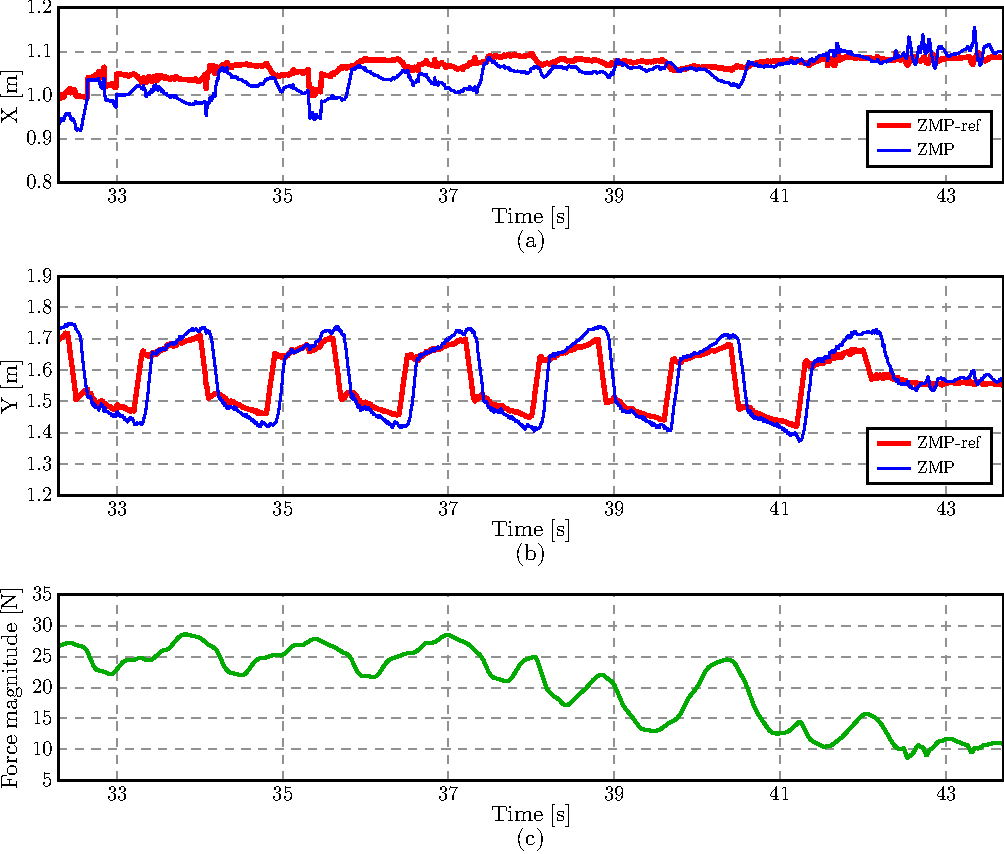
\includegraphics[height=0.40\textwidth]{./figures/exp_ZMP_cont.pdf}
 \vspace{-7mm}
 \caption{Robot's final steps ZMP trajectories in the experiment using the proposed hybrid controller on the left wrist of the robot. In (a) position in $X$ direction, in (b) position in $Y$ direction and in (c) the magnitude of the force applied by the hose on the left wrist.}
 \label{zmp_cont}
% \vspace{-5mm}
\end{figure}
%
%
\begin{figure}[t]
 \centering
 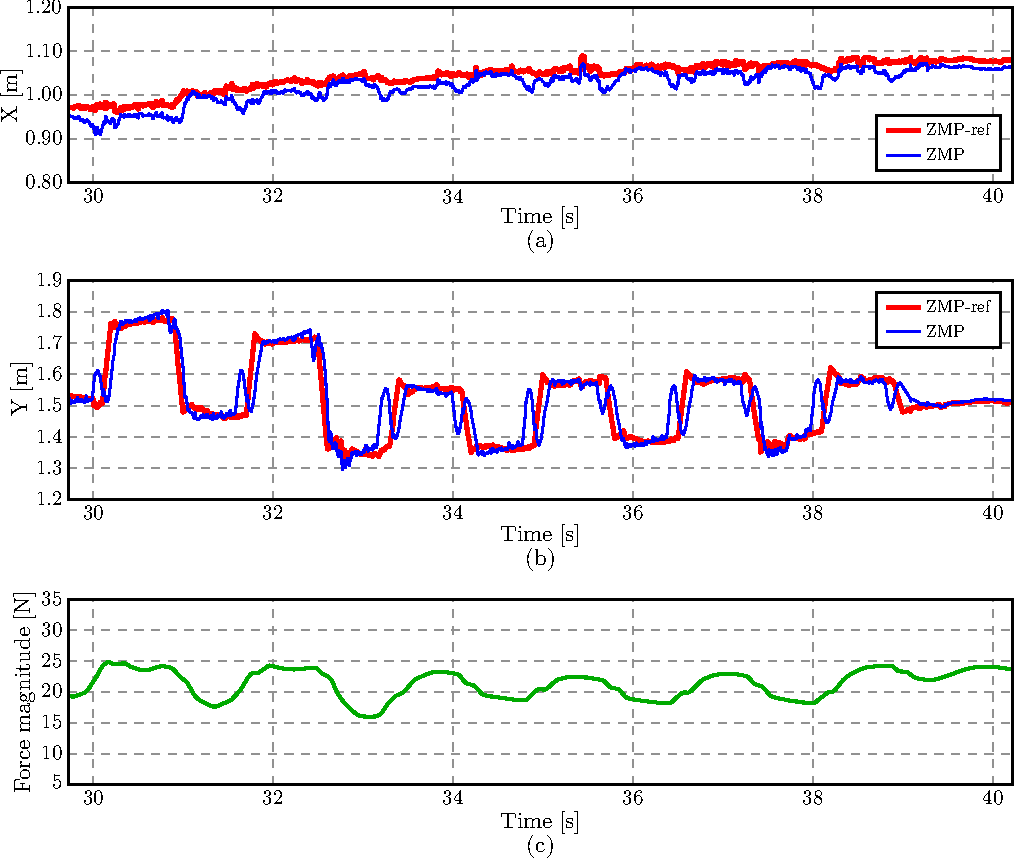
\includegraphics[height=0.37\textwidth]{./figures/exp_ZMP_noCont.pdf}
 \vspace{-7mm}
 \caption{Robot's final steps ZMP trajectories in the experiment with the joint angles of the left arm fixed. In (a) position in $X$ direction, in (b) position in $Y$ direction and in (c) the magnitude of the force applied by the hose on the left wrist.}
 \label{zmp_nocont}
% \vspace{-5mm}
\end{figure}
%

Furthermore, Fig.~\ref{zmp_cont} shows the final steps of the ZMP trajectories of the robot during the experiment, the bold red line represents the reference trajectory computed by the walking pattern generator and the thin blue line represents the real ZMP trajectory computed based on the force sensors of the robot's ankles and the position of the feet.
%
It can be seen that the ZMP, particularly in $Y$ direction, moves away from the reference when the robot is pulling the hose, i.e during the double support phase.
%
This indicates that the robot is losing balance at those points.
%
Nevertheless we were able to successfully reproduce the experiment $4$ times out of $8$ trials. 
%



Fig.~\ref{zmp_nocont} shows the final steps of the ZMP trajectories of the robot for the experiment where no impedance control is being applied to wrist holding the hose i.e. the robot's joint angles of the left arm are fixed.
%
Here, it can be observed that in $Y$ direction the ZMP has rebounds immediately after the left foot has landed on the floor.
%
On the contrary, during with the hybrid controller on the wrist there are no rebounds since the impedance controller is allowing the left arm to absorb part of the disturbance generated by the hose.
%
This means, that the impedance control on the wrist of the robot contributes to the improvement of the robot's balance while walking.
%
